\documentclass[11pt]{article}

\usepackage[portuguese]{babel}
\usepackage[utf8]{inputenc}
\usepackage{amsmath}
\usepackage{graphicx}
\usepackage{float}
\usepackage{subfig}
\usepackage{fixltx2e}
\usepackage{listings}
\usepackage[bottom]{footmisc}
\usepackage{color}
\usepackage{xargs}                      % Use more than one optional parameter in a new commands
\usepackage[pdftex,dvipsnames]{xcolor}  % Coloured text etc.
\usepackage[colorinlistoftodos,prependcaption,textsize=tiny]{todonotes}
\newcommandx{\unsure}[2][1=]{\todo[linecolor=red,backgroundcolor=red!25,bordercolor=red,#1]{#2}}
\newcommandx{\change}[2][1=]{\todo[linecolor=blue,backgroundcolor=blue!25,bordercolor=blue,#1]{#2}}
\newcommandx{\info}[2][1=]{\todo[linecolor=OliveGreen,backgroundcolor=OliveGreen!25,bordercolor=OliveGreen,#1]{#2}}
\newcommandx{\improvement}[2][1=]{\todo[linecolor=Plum,backgroundcolor=Plum!25,bordercolor=Plum,#1]{#2}}
\newcommandx{\thiswillnotshow}[2][1=]{\todo[disable,#1]{#2}}
\usepackage[font=footnotesize]{caption}

\definecolor{keywordcolor}{rgb}{0,0.4,0.7}
\definecolor{commentcolor}{rgb}{0.4,0.4,0.4} 	
\definecolor{mygray}{rgb}{0.5,0.5,0.5} 	% line counter color
\definecolor{mymauve}{rgb}{0.90,0.25,0.47}	% string color
\definecolor{codebackground}{rgb}{0.95,0.95,0.95} 

\lstset{ %
	backgroundcolor=\color{codebackground},   % choose the background color; you must add \usepackage{color} or \usepackage{xcolor}
	basicstyle=\ttfamily \footnotesize,        % the size of the fonts that are used for the code
	breakatwhitespace=false,         % sets if automatic breaks should only happen at whitespace
	breaklines=true,                 % sets automatic line breaking
	captionpos=b,                    % sets the caption-position to bottom
	commentstyle=\color{commentcolor},    % comment style
	deletekeywords={...},            % if you want to delete keywords from the given language
	escapeinside={\%*}{*)},          % if you want to add LaTeX within your code
	extendedchars=true,              % lets you use non-ASCII characters; for 8-bits encodings only, does not work with UTF-8
	keepspaces=true,                 % keeps spaces in text, useful for keeping indentation of code (possibly needs columns=flexible)
	keywordstyle=\color{keywordcolor},       % keyword style
	numbers=left,                    % where to put the line-numbers; possible values are (none, left, right)
	numbersep=5pt,                   % how far the line-numbers are from the code
	numberstyle=\tiny\color{mygray}, % the style that is used for the line-numbers
	rulecolor=\color{black},         % if not set, the frame-color may be changed on line-breaks within not-black text (e.g. comments (green here))
	showspaces=false,                % show spaces everywhere adding particular underscores; it overrides 'showstringspaces'
	showstringspaces=false,          % underline spaces within strings only
	showtabs=false,                  % show tabs within strings adding particular underscores
	stepnumber=1,                    % the step between two line-numbers. If it's 1, each line will be numbered
	%stringstyle=\color{mymauve},     % string literal style
	identifierstyle=\color{mymauve},
	tabsize=2                       % sets default tabsize to 2 spaces
}

\usepackage{titlesec}
\setcounter{secnumdepth}{4}
\titleformat{\paragraph}
{\normalfont\normalsize\bfseries}{\theparagraph}{1em}{}
\titlespacing*{\paragraph}
{0pt}{3.25ex plus 1ex minus .2ex}{1.5ex plus .2ex}

\numberwithin{equation}{section}

\linespread{1.3}
\usepackage{indentfirst}
\usepackage[top=2cm, bottom=2cm, right=2.2cm, left=2.2cm]{geometry}
\addto\captionsportuguese{\renewcommand{\contentsname}{Índice}}

\begin{document}

\begin{titlepage}
\begin{center}

\hfill \break
\hfill \break


\includegraphics[width=0.3\textwidth]{./logo}~\\[1cm]

\textsc{\LARGE Instituto Superior Técnico}\\[0.25cm]
\textsc{\Large Mestrado Integrado em Engenharia Electrotécnica e de Computadores}\\[1.8cm]
\textsc{\huge Arquitecturas Avançadas de Computadores}\\[0.25cm]

{\huge \bfseries Descrição do processador $\mu$Risc a funcionar em \textit{pipeline}\\[1.2cm]}

\begin{tabular}{ l l }
Guilherme Branco Teixeira & \hspace{2mm} n.º 70214 \\ 
Maria Margarida Dias dos Reis & \hspace{2mm} n.º 73099 \\
Nuno Miguel Rodrigues Machado & \hspace{2mm} n.º 74236 
\end{tabular}

\vfill

{\large Lisboa, 10 de Maio 2015} 

\end{center}
\end{titlepage}
 
\pagenumbering{gobble}
\clearpage

\tableofcontents
\pagebreak

\clearpage
\pagenumbering{arabic}

\section{Introdução}

Com este trabalho laboratorial pretende-se projectar um processador $\mu$Risc com funcionamento em \textit{pipeline}. O processador possui 4 andares de \textit{pipelining}: no primeiro andar é feito o \textit{instruction fetch} (IF), no segundo andar é feito o \textit{instruction decode} (ID) e o \textit{operand fetch} (OF), no terceiro andar são executadas operações da ALU (EX) e de acesso à memória de dados (MEM) e, por fim, no quarto é feita a escrita no banco de registos, o \textit{write back }(WB). Com o funcionamento em \textit{pipelining} podem ocorrer dois tipos de conflitos - de dados \textit{(data hazards)} e de controlo \textit{(control hazards)}. 

\todo{estrutura ideal do relatorio: 1:referir no geral que conflitos ha. 2:referir quais os conflitod que temos neste prcessador. 3:referir como os resolvemos. 4:comparar as arquitecturas que testámos. 5:entregar antes da meia-noite LooLoL}

\section{Conflitos associados a uma arquitectura \textit{pipeline}}

\todo{referir nesta seccao explicacoes teoricas dos conflitos que ha. e referir que conflitos ha de facto no nosso processador}

\subsection{Conflitos estruturais}

\subsection{Conflitos de dados}

\todo{aqui por exemplo nos so vamos ter RAW. mas temos de explicar todos os que ha}

\subsection{Conflitos de controlo}
 
\section{Métodos de resolução de conflitos}

Em primeiro lugar apresentam-se os métodos e técnicas de resolução dos conflitos de controlo e dados. Em segundo lugar quais as técnicas que foram de facto utilizadas.

\subsection{Conflitos de dados}

Conflito que surge quando uma instrução depende dos	resultados de uma instrução anterior, de forma a afectar o resultado obtido pela linha de processamento.

\begin{itemize}
	\item \textbf{Solução 1}: Bloqueio dos andares do \textit{pipeline}, \textit{stall}, até que os dados correctos estejam disponíveis;
	\item \textbf{Solução 2}: Se o dado correcto existir algures no \textit{pipeline}, estabelece-se um \textit{bypass} para o andar correcto, aplicando a técnica de \textit{forwarding};
	\vspace{-2.5mm}
	\item \textbf{Solução 3}: Escalonar/reordenar as instruções, se a ordenação for feita pelo compilador, tem-se um escalonamento estático, se for feita pelo \textit{hardware}, escalonamento dinâmico;
\end{itemize}

\subsection{Conflitos de controlo}

Um conflito de controlo surge quando uma instrução de controlo condicional depende dos resultados de uma instrução anterior, de uma forma a impedir um predição correcta. \change{nao impede a prediccao}
\vspace{-2.5mm}
Analisando as soluções apresentadas verificou-se que o escalonamento estático e dinâmico não seria a solução desejada devido a complexidade para um processador de 4 andares comparativamente às outras anteriores. Ponderou-se inicialmente a utilização de \textit{stalls} devido à facilidade de implementação mas devido ao inconveniente de reduzir o número médio de instruções por ciclo, optou-se pela segunda solução de forma a aumentar o número médio de instruções por ciclo como também a complexidade de implementação.

\begin{itemize}
	\item \textbf{Solução 1}: BTB, uma tabela que contém informação sobre os saltos de forma a prever se estes são \textit{taken} ou \textit{not-taken}, previsão esta que é realizada por uma BPB (composta por 1 ou 2 bits), diminuindo assim o número de ciclos desperdiçados em instruções do tipo controlo;
	\item \textbf{Solução 2}: \textit{forwarding} de flags, após se obter o resultado necessário para a predição, establece-se um bypass para verificar a condição do salto;
	\vspace{-2.5mm}
\end{itemize}

\change{explicar o que é uma BTB, explicar BPB}

\section{Estrutura do processador}

\section{Testes de \textit{performance}}

\begin{table}[H]
	\centering
	\caption{\textit{Performance} obtida para os diversos testes com o processador demonstrado na aula.}
	\vspace{-1.5mm}
	\includegraphics[keepaspectratio=true, scale=0.40]{tabelas/processadororiginal}
	\label{tab:processadororiginal}
\end{table}

\begin{table}[H]
	\centering
	\caption{Diversas topologias do processador que foram testadas.}
	\vspace{-1.5mm}
	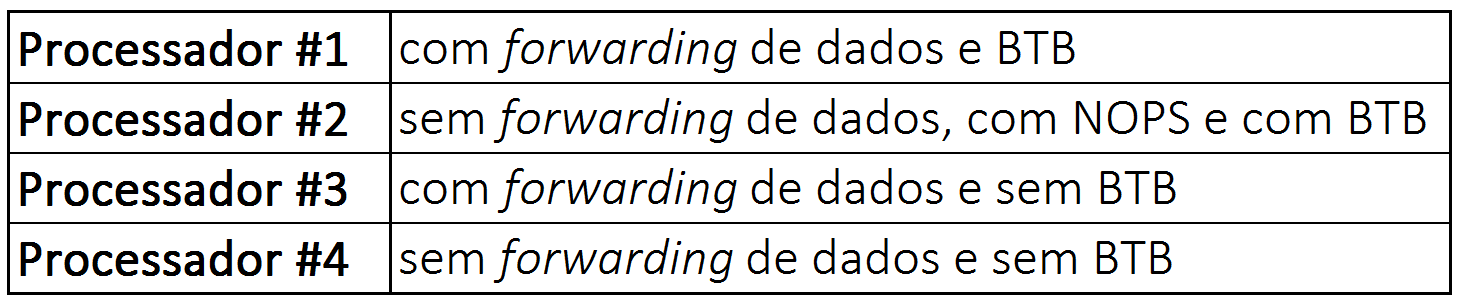
\includegraphics[keepaspectratio=true, scale=0.40]{tabelas/processadores}
	\label{tab:processadores}
\end{table}

\begin{table}[H]
	\centering
	\caption{Resultados obtidos para o teste$\#$1.}
	\vspace{-1.5mm}
	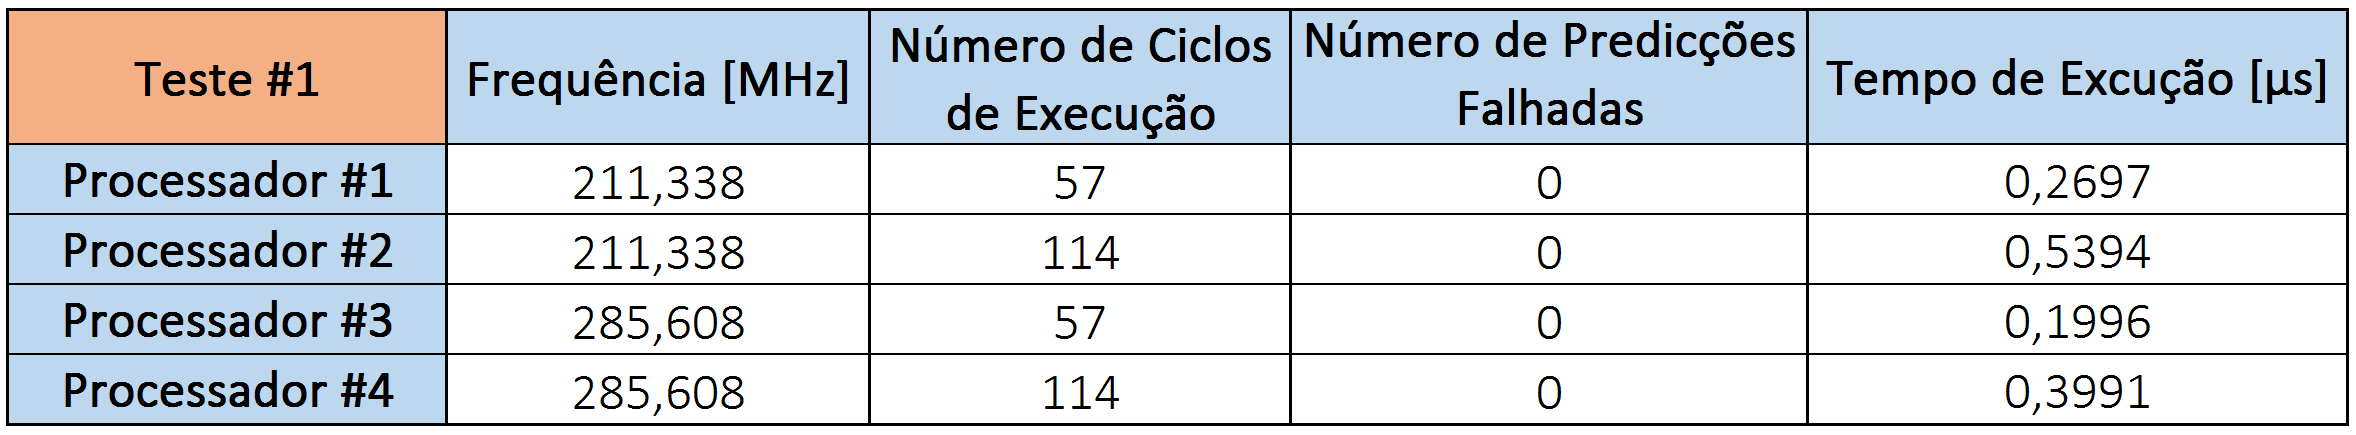
\includegraphics[keepaspectratio=true, scale=0.40]{tabelas/teste1}
	\label{tab:teste1}
\end{table}

\begin{table}[H]
	\centering
	\caption{Resultados obtidos para o teste$\#$2.}
	\vspace{-1.5mm}
	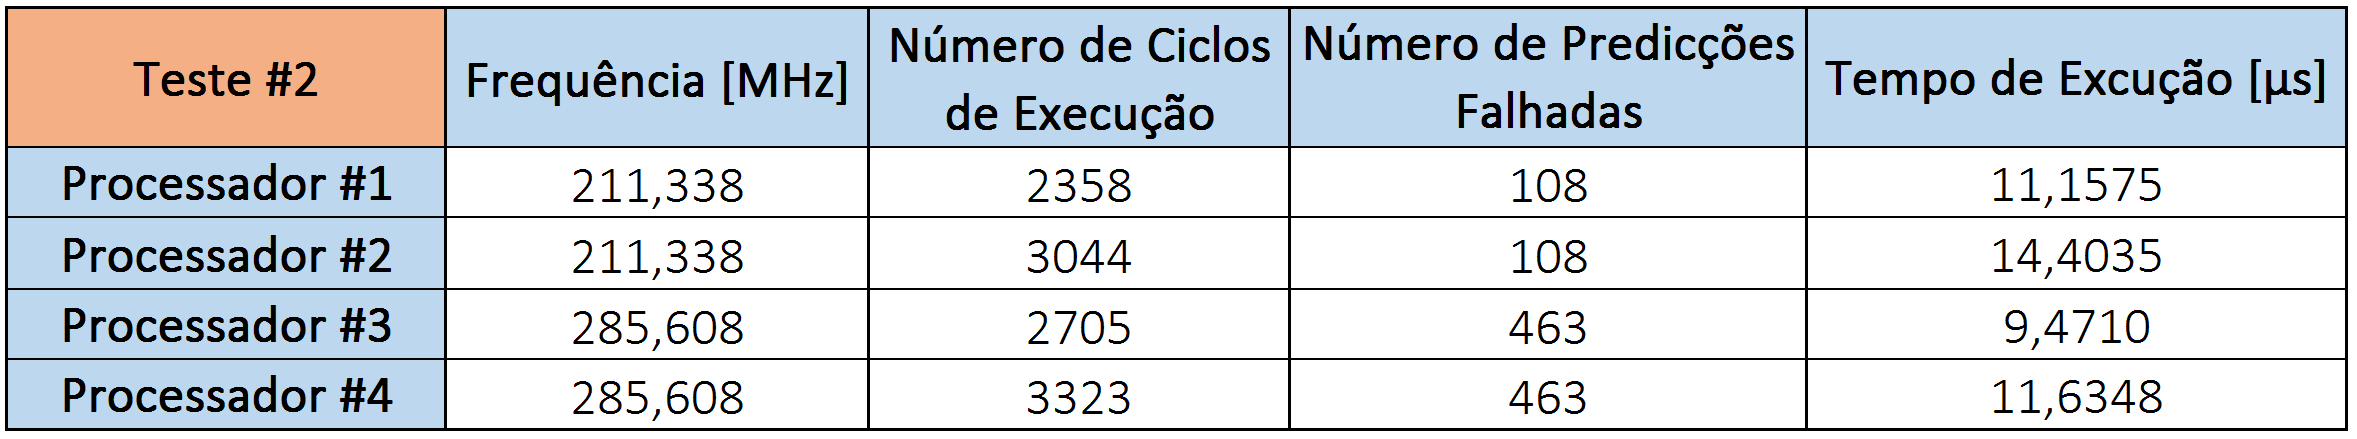
\includegraphics[keepaspectratio=true, scale=0.40]{tabelas/teste2}
	\label{tab:teste2}
\end{table}

\begin{table}[H]
	\centering
	\caption{Resultados obtidos para o teste$\#$3.}
	\vspace{-1.5mm}
	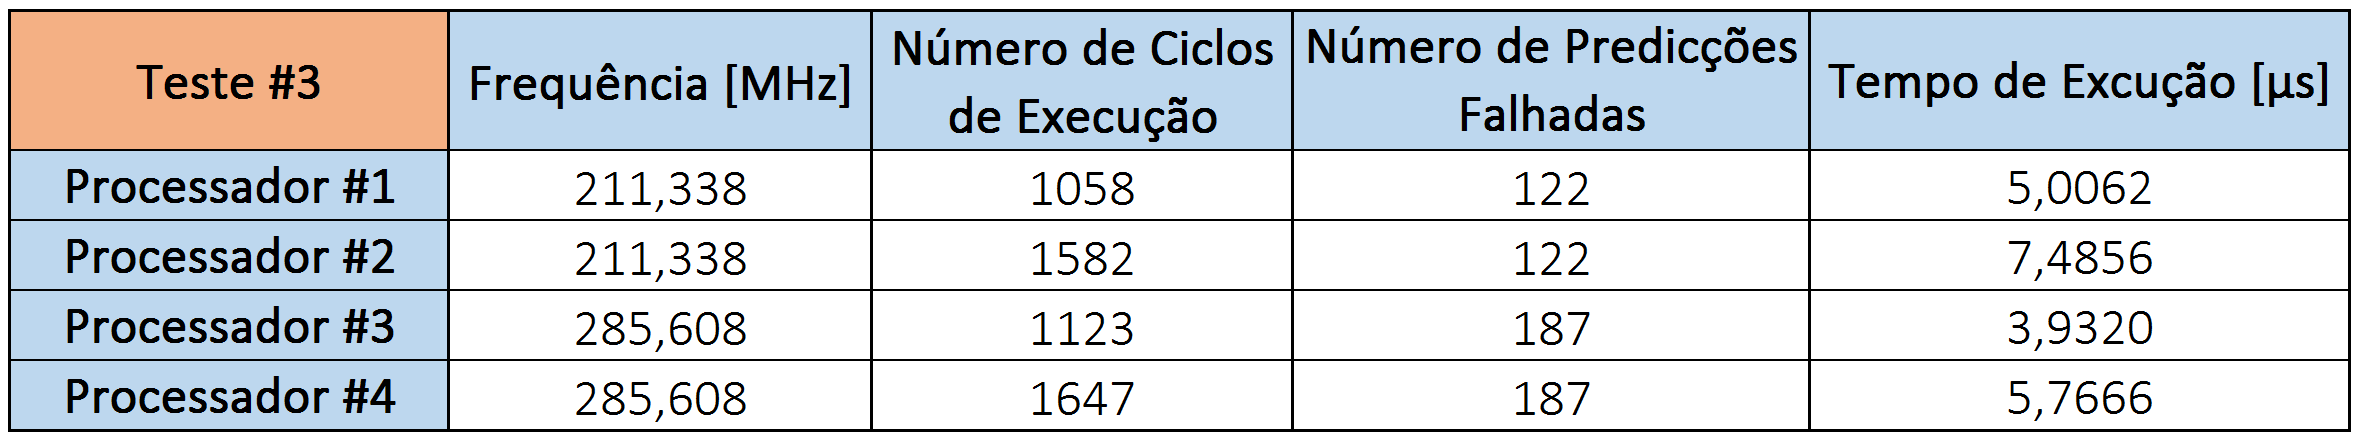
\includegraphics[keepaspectratio=true, scale=0.40]{tabelas/teste3}
	\label{tab:teste3}
\end{table}

\section{Conclusões}

\pagebreak

\section{Anexos}

\subsection{Código do andar de IF}

\lstinputlisting[language=VHDL]{IF.vhd}

\subsection{Código do andar de ID e OF}

\lstinputlisting[language=VHDL]{IDeOF.vhd}

\subsection{Código do andar de EX e MEM}

\lstinputlisting[language=VHDL]{EXeMEM.vhd}

\subsection{Código do andar de WB}

\lstinputlisting[language=VHDL]{WB.vhd}

\subsection{Código da memória ROM}

\lstinputlisting[language=VHDL]{memoria_ROM.vhd}

\subsection{Código da memória RAM}

\lstinputlisting[language=VHDL]{memoria_RAM.vhd}

\subsection{Código da BTB}

\lstinputlisting[language=VHDL]{BTB_bram.vhd}

\subsection{Código da máquina de estados}

\lstinputlisting[language=VHDL]{Controlo.vhd}

\pagebreak

\listoftodos

\end{document}